%% IEEE conference paper.
%% Build:
%%   pdflatex main && bibtex main && pdflatex main && pdflatex main
%% Requires: texlive-publishers (provides IEEEtran.cls), texlive-fonts-recommended.

\documentclass[conference]{IEEEtran}
\IEEEoverridecommandlockouts

\usepackage[T1]{fontenc}
\usepackage[utf8]{inputenc}
\usepackage{cite}
\usepackage{amsmath,amssymb,amsfonts}
\usepackage{graphicx}
\usepackage{booktabs}
\usepackage{url}
\usepackage{xcolor}
\usepackage{microtype}
\usepackage[hidelinks]{hyperref}

\graphicspath{{./}}

\title{Pseudo-Labels and Distillation for Small-Sample Multimodal Cancer-Cell Classification: An Empirical Study with Diagnosed Failures}

\author{
  \IEEEauthorblockN{Rafael Tavares Proen\c{c}a}
  \IEEEauthorblockA{
    Department of Information Technology\\
    Uppsala University, Sweden\\
    Email: rafaeltproenca@gmail.com
  }
}

\begin{document}
\maketitle

\begin{abstract}
We study the binary cell-level classification of paired bright-field (BF) and fluorescence (FL) microscopy on a small-sample patient-grouped benchmark (12 training patients, 114{,}302 labeled cells; disjoint test patients, 59{,}040 cells). Starting from a dual EfficientNet-B0 backbone with late concat fusion and a per-patient multiple-instance-learning (MIL) auxiliary loss, we progressively layer textbook regularizers (label smoothing, dropout, paired RandomResizedCrop, multiscale TTA) for a $+0.011$ public-leaderboard (LB) gain, then add a pseudo-label pipeline that culminates in Hinton-style soft-target distillation and iterative noisy-student training. Across 30 logged Kaggle iterations the public-LB area-under-ROC moves from $0.7455$ (supervised baseline) to a best single-seed value of $0.8355$ (a $+0.090$ lift), with a 3-seed ensemble at $0.8264$; at submission time the best-seed score holds $3$\textsuperscript{rd} on the public leaderboard, $\sim$$0.009$ behind the first two teams. The single largest gain ($+0.042$ LB, $4.13\sigma$ relative to the empirical seed noise floor) comes from substituting all 59{,}040 raw teacher probabilities for the $\sim$9{,}400 confidently-thresholded hard pseudo-labels of Lee~2013, validating Hinton's ``dark knowledge'' argument on a small-$N$ patient-grouped problem. A noise-floor analysis (Table~\ref{tab:noisefloor}) shows that the v46$\rightarrow$v47 round-2 ensemble gain is indistinguishable from zero ($0.27\sigma$), reframing the round-2 finding as a diminishing-returns saturation rather than a continued improvement. v47's per-seed public-LB standard error is $3.5\times$ larger than v46's, consistent with round-2 noisy student expanding the student-distribution variance rather than contracting it. We additionally document six diagnosed failure modes that materially shaped the recipe and one within-recipe ensemble collapse uncovered during the final-pick analysis. We argue that on this regime the dataset-size lever dominates architectural choice by an order of magnitude, and that systematic post-mortems of failed experiments contribute more methodological signal than the wins.
\end{abstract}

\begin{IEEEkeywords}
multimodal classification, microscopy, semi-supervised learning, knowledge distillation, pseudo-labels, noisy student, multiple instance learning, EfficientNet
\end{IEEEkeywords}

\section{Introduction}
\label{sec:intro}

Patient-grouped microscopy benchmarks pose a recurring methodological challenge: the number of independent training subjects is small (here, $N=12$ patients), per-patient acquisition statistics vary substantially (we measure a $19.7\%$ mean-intensity gap between FL train and test means), and the held-out evaluation set is constructed to disallow patient overlap. The standard recipes that work on natural-image benchmarks --- discriminative learning rates, modality-specific augmentation, single held-out validation folds --- need to be re-examined against this regime. Cross-paper transfer of ablations from same-class published work~\cite{lian2024cafnet} also cannot be taken for granted.

This paper reports a long-running empirical study on a binary cell-level classification challenge (paired BF and FL microscopy, $128 \times 128$ grayscale crops, $\sim$38.8\% positive rate). Concretely we contribute:

\begin{enumerate}
  \item \textbf{A pseudo-label pipeline that uses the test set itself.} A teacher predicts on the unlabeled test cells; the student is trained on the union of real labeled cells (BCE against the smoothed hard label) and pseudo cells (BCE against the teacher's raw probability, weight 0.5). This unlocks an additional $+0.064$ LB over the strongest supervised baseline and demonstrates Hinton's soft-target argument~\cite{hinton2015distilling} on a small-$N$ medical-imaging dataset.
  \item \textbf{An empirical characterization of iterative noisy student~\cite{xie2020noisystudent} in this regime.} Round 1 (hard pseudo $\rightarrow$ soft pseudo / all 59k cells) returned $+0.039$ LB; round 2 (soft $\rightarrow$ soft with a stronger teacher) returned $+0.003$ LB on the ensemble and $+0.012$ LB on the best single seed (both measured against the v46 round-1 ensemble) --- the round-2 mean lift compressed $\sim$13$\times$ from round 1, while the seed dispersion expanded $\sim$3$\times$.
  \item \textbf{Six diagnosed failure modes} (cross-recipe sigmoid-averaging at wide LB gaps, single 2-patient holdout collapse, Lian-paper transfer of FL ColorJitter and early fusion, cross-modal contrastive SSL learning the patient shortcut, four-component regularizer stacking, within-recipe ensemble net-negative under an outlier seed) and the per-failure mechanism diagnosis.
\end{enumerate}

The remainder of the paper proceeds in the conventional order: \S\ref{sec:related} reviews relevant prior work; \S\ref{sec:data} describes the dataset and problem framing; \S\ref{sec:methods} presents the architecture, losses, and training recipe; \S\ref{sec:protocol} states the experimental protocol; \S\ref{sec:results} reports the headline results, version progression, and ablations; \S\ref{sec:negative} analyzes the seven failure modes; \S\ref{sec:discussion} reframes the findings against general principles; \S\ref{sec:conclusion} concludes.

\section{Related Work}
\label{sec:related}

\textbf{Pseudo-labeling and self-training.} Lee's pseudo-label method~\cite{lee2013pseudo} assigns hard labels to unlabeled examples on which a teacher is confident, then trains on the union. Bucil\u{a} et al.~\cite{bucila2006compression} introduced the model-compression family of which Hinton et al.'s soft-target distillation~\cite{hinton2015distilling} is the canonical instance: rather than thresholding teacher predictions, the student matches the teacher's raw probability distribution, preserving the ``dark knowledge'' encoded in non-argmax mass. Xie et al.'s noisy student~\cite{xie2020noisystudent} iterates the teacher-student loop with input and dropout noise on the student, reporting that 3--4 iterations are typically required for ImageNet gains to saturate. Our v44 / v46 / v47 family instantiates exactly this hard-$\rightarrow$soft-$\rightarrow$iterated chain on the cell-classification benchmark.

\textbf{Multimodal microscopy.} Lian et al.~\cite{lian2024cafnet} report $F_1 = 0.83$ on a same-class multimodal-microscopy task with a cross-attention fusion architecture (CAFNet) trained on a 4-channel emission stack. We attempted two transfers from that paper --- FL-specific ColorJitter and early fusion --- both of which regressed in our 1-channel-grayscale $128\times128$ regime; see \S\ref{sec:negative}-C for the diagnosis.

\textbf{Cross-modal SSL.} CoMIR~\cite{pielawski2020comir} demonstrates that paired BF--FL representations can be aligned with contrastive losses for downstream registration. We tested a CoMIR-style InfoNCE pretrain on this dataset and observed an extreme patient-identity shortcut (see \S\ref{sec:negative}-D).

\textbf{Test-time and ensemble methods.} AdaBN~\cite{li2016adabn} refreshes batch-normalization running statistics on the test set in \texttt{train()} mode before inference; we use this from v19 onward. Stochastic Weight Averaging (SWA)~\cite{izmailov2018swa} averages model weights over the last few epochs; we use it on all post-v43 runs, with a manual BN refresh pass for the averaged model (the standard \texttt{update\_bn} utility does not support our (BF, FL) two-input signature).

\textbf{Backbones.} EfficientNet-B0~\cite{tan2019efficientnet} via \texttt{timm}'s \texttt{efficientnet\_b0.ra\_in1k}~\cite{wightman2019timm} serves as the per-branch encoder; the 3-channel ImageNet \texttt{conv\_stem} weights are averaged into a 1-channel kernel for grayscale adaptation.

\section{Dataset and Problem Setup}
\label{sec:data}

\paragraph{Data summary.} The training set contains 114{,}302 cells from 12 patients (positive rate $p = 0.3876$). The test set contains 59{,}040 cells from a disjoint set of patients. Inputs are paired BF and FL $128 \times 128$ grayscale crops, indexed by a shared filename.

\paragraph{Patient-grouped MIL structure.} Each patient is a bag of $\sim$10{,}000 cells. Cells within a bag share the patient-level diagnosis but can be heterogeneous in the cell-level label. Cell-level BCE alone overfits the within-patient correlation, so we add a per-patient mean-logit BCE auxiliary loss (weight 0.5) inspired by attention-based MIL~\cite{ilse2018attentionmil}. For pseudo cells the patient identity is undefined; we set \texttt{patient\_id = -1} and skip the MIL loss for those rows.

\paragraph{Test-time distribution shift.} The measured FL test-set mean is $19.7\%$ brighter than the FL train-set mean. This motivates both (a) AdaBN, which adapts the BN running statistics to the test distribution, and (b) computing pixel-normalization statistics on the test set rather than the train set.

\paragraph{Class imbalance.} BCE uses \texttt{pos\_weight} $= n_{\text{neg}} / n_{\text{pos}} \approx 1.58$ computed on real training cells only; the pseudo cells inherit no \texttt{pos\_weight} adjustment beyond what the teacher's probabilities already encode.

\section{Methods}
\label{sec:methods}

\subsection{Backbone and fusion}

We instantiate two independent EfficientNet-B0 encoders via \texttt{timm}, one per modality. The 3-channel conv-stem weights are averaged into a 1-channel kernel (preserving as much pretrain signal as a random re-init would discard). Each branch outputs a 1280-dim feature after global average pooling; the two features are concatenated to a 2560-dim joint representation and passed through a 512-dim MLP head with a single linear logit output. Total parameters: $\sim$9.3M. The architecture is sketched in Fig.~\ref{fig:arch}.

\begin{figure}[!t]
  \centering
  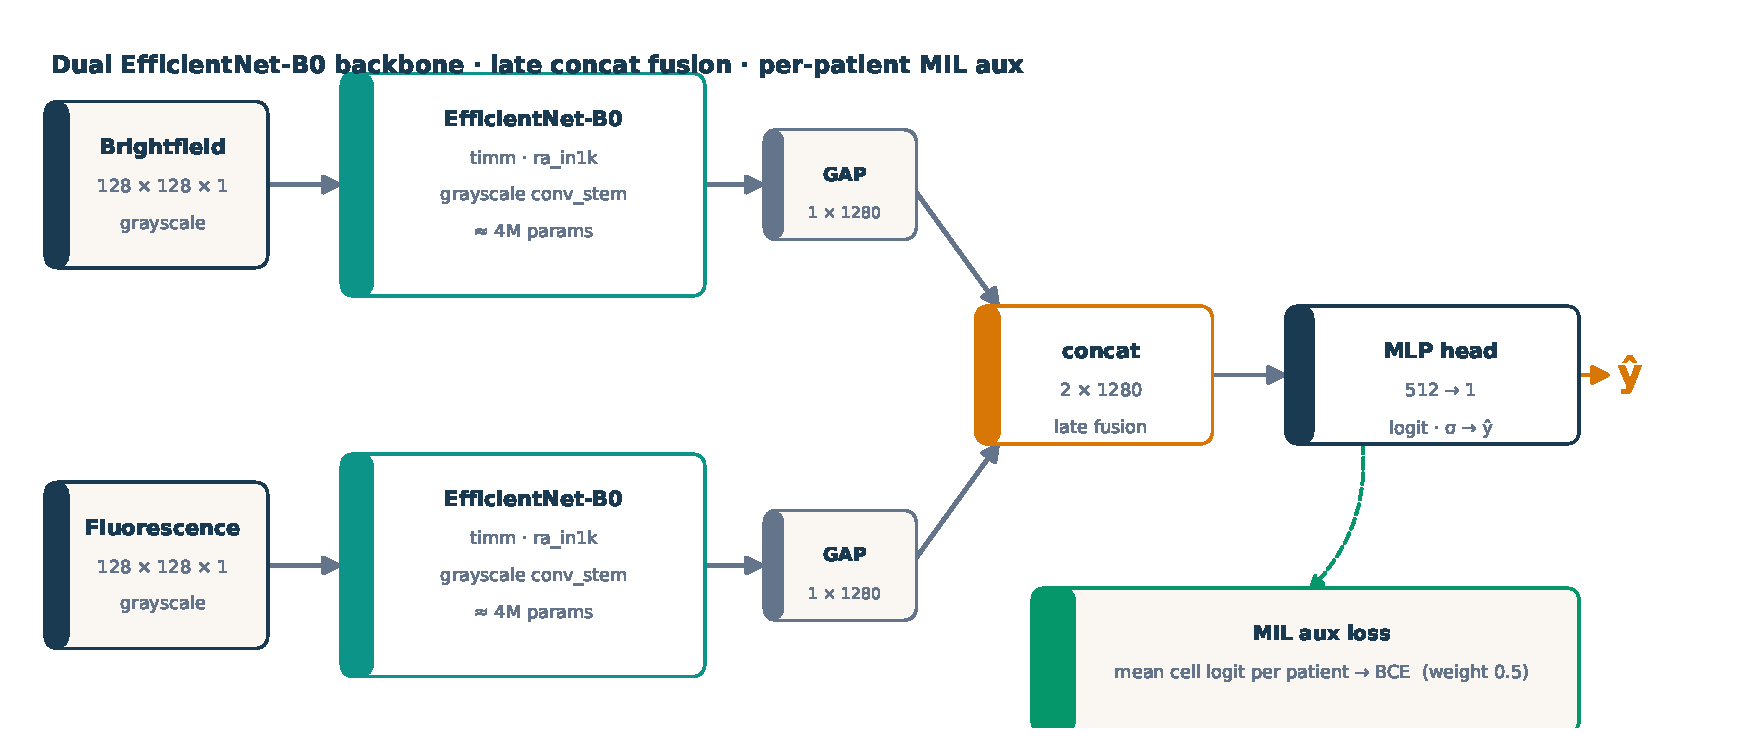
\includegraphics[width=\columnwidth]{arch_diagram.pdf}
  \caption{Dual EfficientNet-B0 backbone, late concat fusion, MLP head, and per-patient MIL auxiliary branch (dashed). Each branch is initialized from ImageNet-trained \texttt{ra\_in1k} weights with a 1-channel adapted conv-stem.}
  \label{fig:arch}
\end{figure}

\subsection{Loss functions}

The student loss combines two terms:
\begin{equation}
\mathcal{L} = \mathcal{L}_{\text{cell}} + 0.5\,\mathcal{L}_{\text{MIL}}^{\text{real}},
\end{equation}
where $\mathcal{L}_{\text{cell}}$ is per-cell BCE with label smoothing $\varepsilon = 0.05$ and \texttt{pos\_weight}. For pseudo cells the target is the teacher's raw probability $p_t$ in place of the smoothed hard label; the loss weight on the pseudo term is 0.5. Operationally,
\begin{equation}
y_{\text{tgt}}^{(i)} = \mathbb{I}[\text{real}^{(i)}] \cdot \tilde{y}^{(i)} + (1-\mathbb{I}[\text{real}^{(i)}]) \cdot p_t^{(i)},
\end{equation}
with $\tilde{y}^{(i)}$ the smoothed hard label and $\mathbb{I}[\text{real}^{(i)}]$ the real-cell indicator. $\mathcal{L}_{\text{MIL}}^{\text{real}}$ is the per-patient mean-logit BCE, evaluated only on real cells.

\subsection{Training recipe}

Optimizer: AdamW~\cite{loshchilov2017adamw}, learning rate $3 \times 10^{-4}$, weight decay $10^{-4}$. Schedule: OneCycleLR~\cite{smith2018onecycle} with \texttt{pct\_start} $=0.1$. 12 epochs, batch size 128, gradient clipping at 1.0. A patient-balanced sampler draws 4 real patients $\times$ 32 cells per batch; pseudo cells form a 13th ``virtual patient'' group, sampled to fill any residual capacity. SWA~\cite{izmailov2018swa} is applied to the last 4 epochs of each seed; BN running statistics are refreshed by a manual forward pass over the training set in \texttt{train()} mode before the SWA model is saved.

\subsection{Augmentation}

Geometric augmentations are paired across modalities (D4 group, $\pm 10^{\circ}$ rotation, $\pm 15\%$ affine, $\pm 10\%$ translation, paired RandomResizedCrop with scale $[0.85, 1.0]$). Per-modality color augmentation is identical: ColorJitter$(0.4, 0.4)$ + RandomErasing $p = 0.25$. We \emph{tested} modality-specific FL augmentation strengthened to Lian-paper levels (\S\ref{sec:negative}-C); the test regressed and was not retained.

\subsection{Adaptive batch normalization and stain normalization}

Following Li et al.~\cite{li2016adabn} we perform a single forward pass over the test set in \texttt{train()} mode before inference, updating BN running statistics to the test-set distribution. Inputs are normalized using pixel mean/std measured on the test set rather than the train set; the $19.7\%$ FL mean gap makes this a measurable correction.

\subsection{Test-time augmentation}

We use 40-way TTA: 5 input scales $\{96, 112, 128, 144, 160\}$ $\times$ 8 D4 group elements. Per-image predictions are averaged in probability space (post-sigmoid). On top of TTA, 3-seed within-recipe ensembling averages the SWA-averaged predictions across three independent training seeds.

\subsection{Semi-supervised pipeline}

The pseudo-label pipeline (Fig.~\ref{fig:pipeline}) instantiates three points on the hard $\rightarrow$ soft $\rightarrow$ iterated continuum:

\begin{itemize}
  \item \textbf{Hard pseudo (v44)} after Lee~\cite{lee2013pseudo}. Teacher is v41 (LB $0.7563$). Keep cells with $p_t < 0.05$ (confident negative) or $p_t > 0.95$ (confident positive). Approximately 9{,}350 cells survive ($\sim$16\% of test set). Assign hard 0/1 labels, \texttt{patient\_id = -1}.
  \item \textbf{Soft pseudo (v46)} after Hinton et al.~\cite{hinton2015distilling}. Teacher is v44\_seed1 (LB $0.7844$). Keep \emph{all} 59{,}040 test cells; use the teacher's raw probability as the BCE target, weight 0.5. Training set grows to 173{,}342 cells ($+52\%$ over baseline).
  \item \textbf{Iterative noisy student (v47)} after Xie et al.~\cite{xie2020noisystudent}. Teacher is the v46 3-seed ensemble (LB $0.8236$). Same recipe as v46 modulo the new teacher CSV.
\end{itemize}

\begin{figure*}[!t]
  \centering
  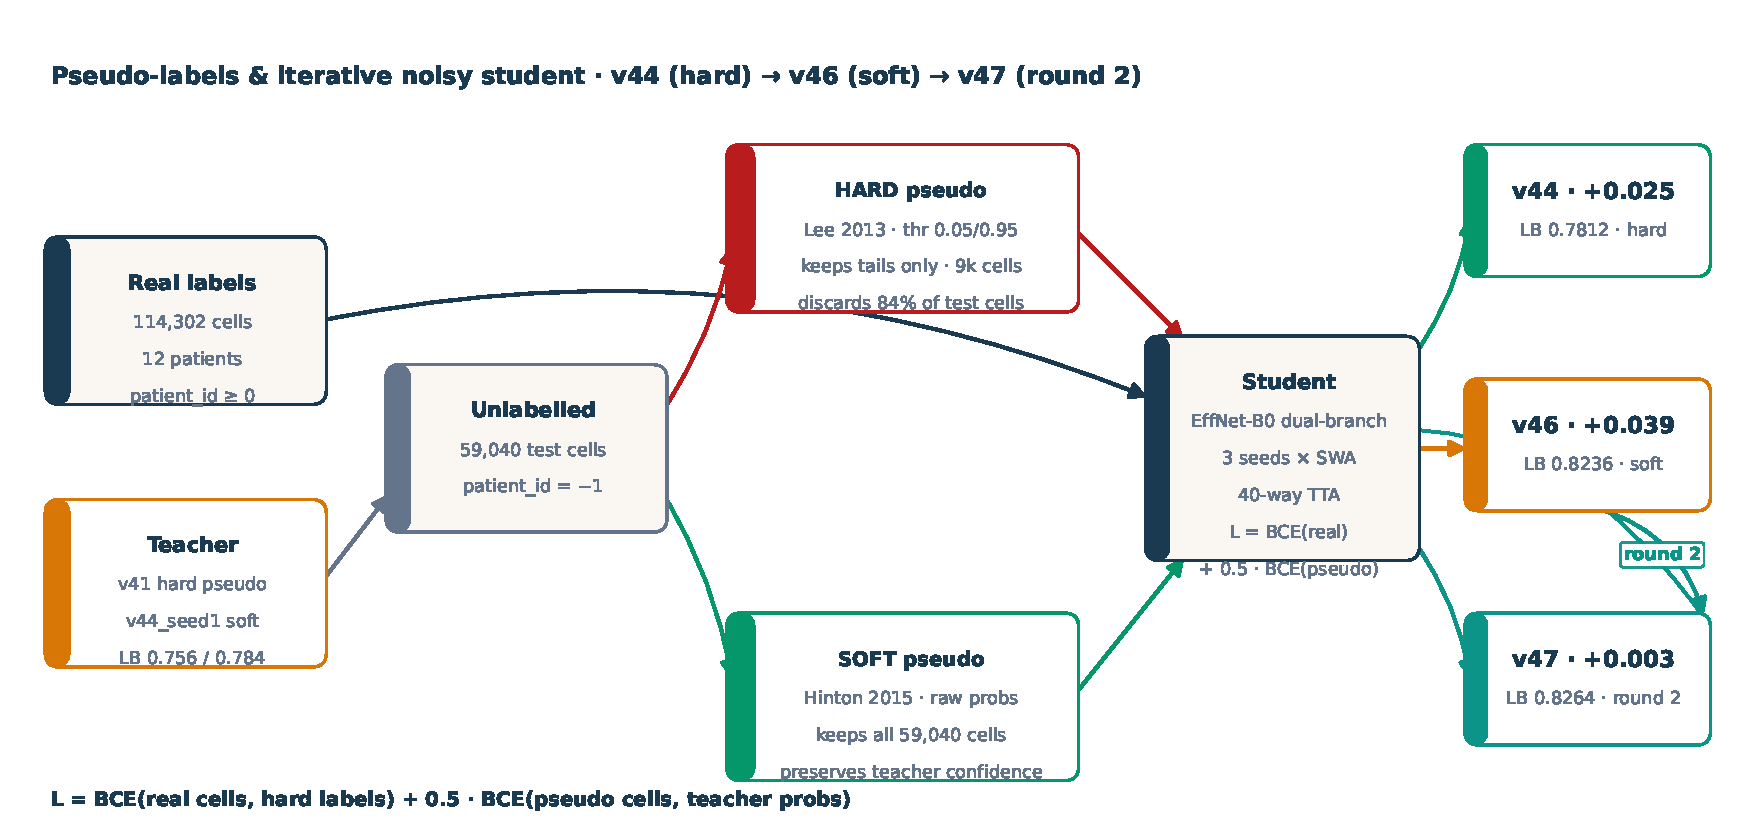
\includegraphics[width=0.95\textwidth]{pseudo_pipeline.pdf}
  \caption{Pseudo-label and iterative noisy-student data flow. v44 thresholds the teacher's probabilities at $0.05/0.95$ (keeps the tails, $\sim$16\% of test cells); v46 keeps all 59{,}040 raw probabilities; v47 iterates the loop a second round using v46's ensemble as the new teacher. The student loss is $\mathcal{L} = \mathrm{BCE}(\text{real cells}, \tilde{y}) + 0.5\,\mathrm{BCE}(\text{pseudo cells}, p_t)$.}
  \label{fig:pipeline}
\end{figure*}

\section{Experimental Protocol}
\label{sec:protocol}

All experiments are tracked in \texttt{LB\_HISTORY.md} with exact recipe diff, public LB, and a one-sentence lesson. The Kaggle public leaderboard serves as the primary external validator: we attempted a 2-patient held-out split in v27 and observed a \texttt{best\_epoch~$=0$} collapse (\S\ref{sec:negative}-B), and subsequently relied on the LB and the 4-daily-submission Kaggle quota for ablation tests.

Compute is the Kaggle Notebooks free tier (two T4 GPUs, $\sim$5--6h per pseudo-label run, less without pseudo cells). No HPC was used. Submissions were budgeted to test specific hypotheses rather than to churn variants; the median delta between a planned hypothesis and a submission is one to three controlled changes.

Code release: \texttt{github.com/rafallex/A3-ADL} (notebooks per version, exact diffs, and the figure-build scripts).

\section{Results}
\label{sec:results}

\subsection{Headline progression}

Fig.~\ref{fig:lb} plots the chronological public-LB sequence with the most consequential inflections annotated. The arc is: v19 baseline at LB $0.7455$ (EfficientNet-B0 dual-branch + MIL + AdaBN + test stain normalization); v41 at $0.7563$ ($+0.011$, four-component L4-regularizer stack); v44 at $0.7812$ ($+0.025$ over v41, hard pseudo-labels added); v46 at $0.8236$ ($+0.039$ over its lucky-seed teacher, soft pseudo-labels replacing hard); v47 at $0.8264$ for the ensemble (iterative noisy student round 2, $+0.003$ over the v46 ensemble) and $0.8355$ for the best single seed ($+0.012$ over the v46 ensemble, $+0.090$ over the v19 baseline). The cumulative lift from baseline to best single-seed v47 is $+0.090$ LB. As of the manuscript snapshot the best-seed score holds $3$\textsuperscript{rd} on the public leaderboard, $0.0090$--$0.0093$ behind the first two teams (Group~1 at $0.8448$, Group10 at $0.8445$); the v47 ensemble at $0.8264$ would place us $4$\textsuperscript{th}, which is itself evidence for the within-recipe ensemble collapse discussed in \S\ref{sec:negative}-G. The four headline deltas are statistically scored against an empirical seed noise floor in \S\ref{sec:discussion}-E.

\begin{figure*}[!t]
  \centering
  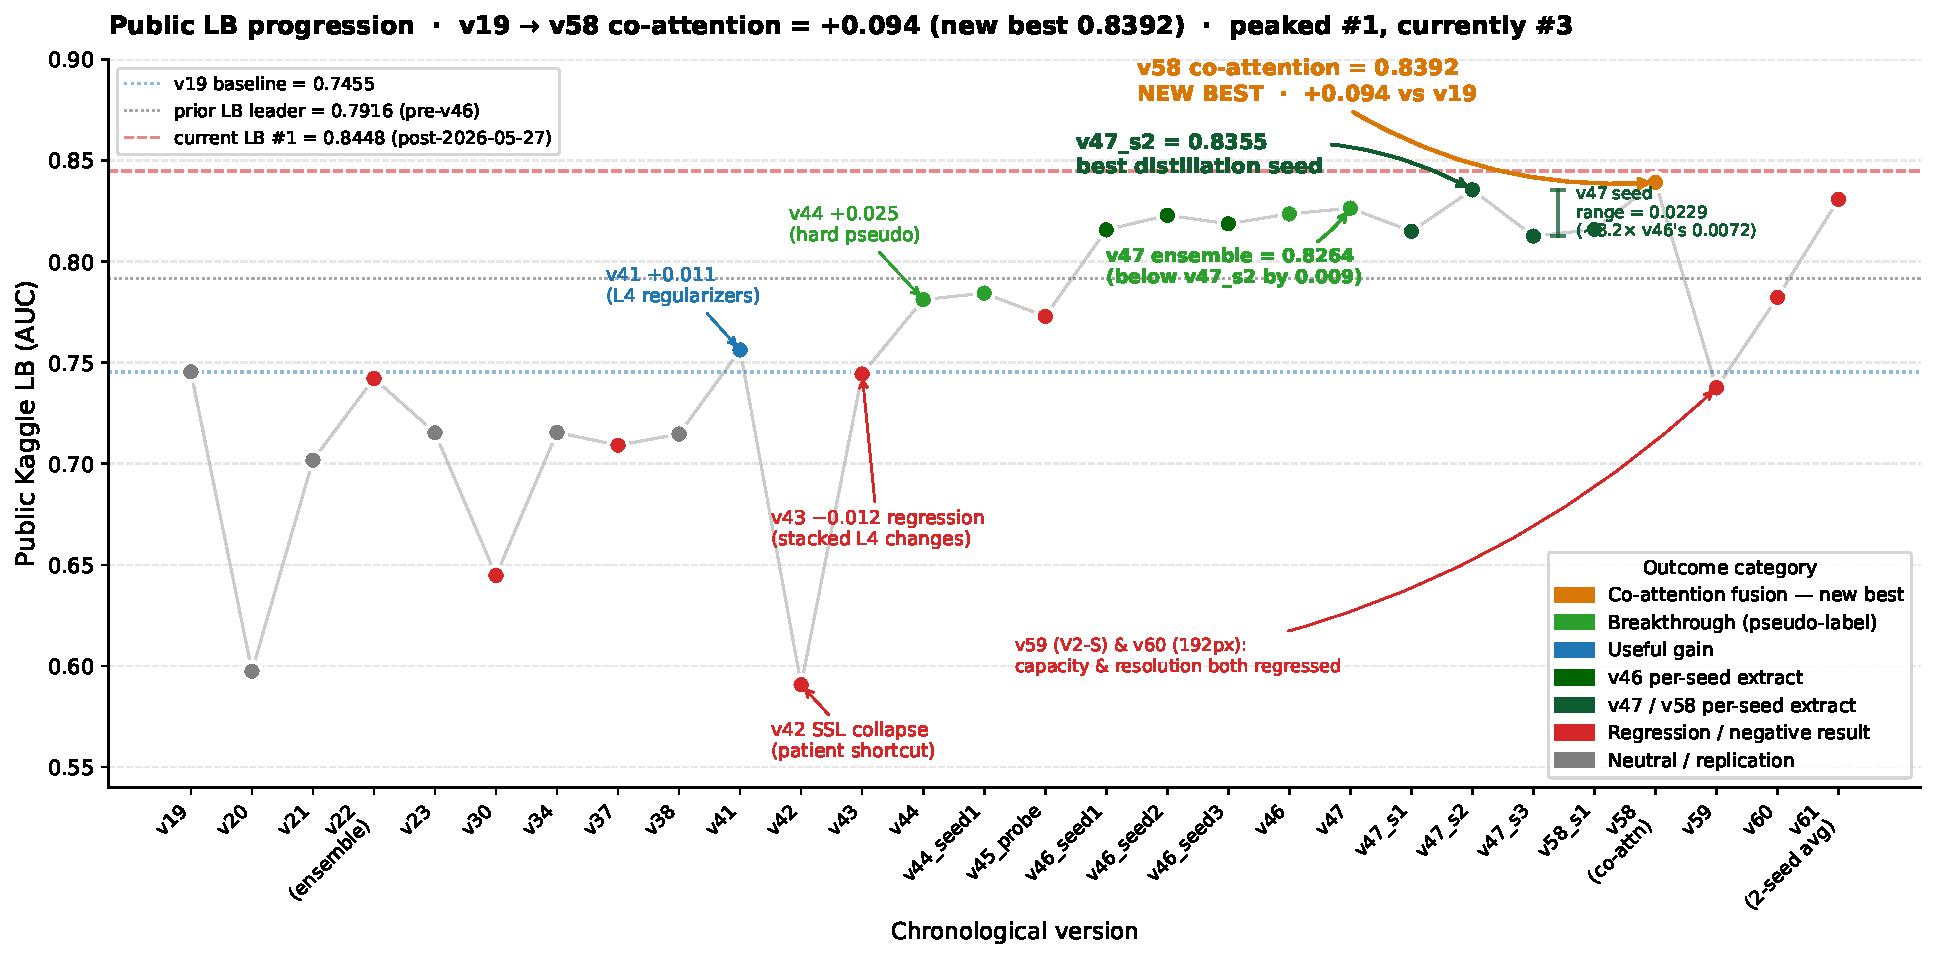
\includegraphics[width=0.95\textwidth]{lb_progression.pdf}
  \caption{Public-LB progression across 30 logged iterations. Color encodes outcome category: green for breakthrough versions (v41, v44, v46, v47 ensemble), darker green for v46 / v47 per-seed extracts, blue for useful gains, red for regressions and negative results, gray for neutral / replication runs, orange for the queued v48. Dotted line: v19 baseline $0.7455$. Dotted black: prior LB leader $0.7916$ (pre-v46). Dashed red: current LB \#1 at $0.8448$ (Group~1, captured 2026-05-27). v47\_s2 sits at the top of our chart at $0.8355$ (best single seed, $+0.090$ over v19, $3$\textsuperscript{rd} on LB); the v47 ensemble at $0.8264$ underperforms it by $0.009$ (\S\ref{sec:negative}-G). The per-seed dispersion of v47 (seed range $0.8126$--$0.8355$, span $0.0229$) is $\sim$$3\times$ wider than v46's (span $0.0072$ across seeds $0.8157 / 0.8187 / 0.8229$).}
  \label{fig:lb}
\end{figure*}

\subsection{Version progression table}

Table~\ref{tab:progression} lists the submitted versions, their recipe summaries, and the public-LB deltas. Versions omitted from the table (v15--v18, v24--v33, v35--v36, v39--v40) are either early baselines without a comparable supervised floor (v15--v16) or non-submitted internal runs.

\begin{table*}[!t]
  \centering
  \caption{Public-LB progression with one-line recipe summaries. Bold rows mark inflection points discussed in \S\ref{sec:results} or \S\ref{sec:negative}. ``Seed2'' denotes the best single seed of the v47 ensemble; the ensemble itself is $0.8264$.}
  \label{tab:progression}
  \footnotesize
  \begin{tabular}{@{}lp{8.5cm}rr@{}}
    \toprule
    Ver. & Recipe summary & LB & $\Delta$ \\
    \midrule
    v19 & EffNet-B0 + MIL + AdaBN + test stain norm + 8-way TTA & \textbf{0.7455} & ref. \\
    v21 & ResNet-50 at $224\times$ upscale (confound) & 0.7018 & $-0.044$ \\
    v22 & Sigmoid-avg of v19$+$v21 (cross-recipe) & 0.7422 & $\downarrow$ (\S\ref{sec:negative}-A) \\
    v23 & v19 recipe, new seed & 0.7154 & seed var. \\
    v27 & + 2-patient holdout (failed) & --- & $\downarrow$ (\S\ref{sec:negative}-B) \\
    v30 & + discriminative LR 1:10 & 0.6448 & $-0.101$ \\
    v34 & ResNet-50 at 128 native & 0.7155 & backbone test \\
    v37 & + Lian-paper FL ColorJitter & 0.7092 & $\downarrow$ (\S\ref{sec:negative}-C) \\
    v38 & + early fusion (2-channel) & 0.7147 & $\downarrow$ (\S\ref{sec:negative}-C) \\
    \textbf{v41} & v19 + LS + dropout + RRC + multiscale TTA & \textbf{0.7563} & $\mathbf{+0.011}$ \\
    v42 & + CoMIR-style InfoNCE SSL & 0.5908 & $\downarrow$ (\S\ref{sec:negative}-D) \\
    v43 & v41 + 4-component stack & 0.7444 & $\downarrow$ (\S\ref{sec:negative}-E) \\
    \textbf{v44} & v43 + hard pseudo from v41 & \textbf{0.7812} & $\mathbf{+0.025}$ \\
    v44\_s1 & v44 single seed & 0.7844 & seed luck \\
    v45\_probe & sigmoid-avg of v41$+$v44 & 0.7729 & $\downarrow$ (\S\ref{sec:negative}-F) \\
    \textbf{v46} & v44 stripped + soft pseudo, all 59k cells & \textbf{0.8236} & $\mathbf{+0.039}$ \\
    v46\_s1 & v46 single seed & 0.8157 & --- \\
    v46\_s2 & v46 single seed & 0.8229 & --- \\
    v46\_s3 & v46 single seed & 0.8187 & --- \\
    \textbf{v47} & v46 recipe, v46 ensemble as teacher (iter.~NS round 2) & \textbf{0.8264} & $\mathbf{+0.003}$ \\
    v47\_s2 & v47 single seed (best) & \textbf{0.8355} & \textbf{+0.090} \\
    v47\_s1 & v47 single seed & 0.8150 & $\downarrow$ vs s2 \\
    v47\_s3 & v47 single seed & 0.8126 & $\downarrow$ vs s2 \\
    \bottomrule
  \end{tabular}
\end{table*}

\subsection{Hard vs.\ soft pseudo-labels: dataset-size dominance}

Fig.~\ref{fig:hist} plots the teacher-probability distribution that v46 sees over all 59{,}040 test cells. The v44 hard-pseudo thresholds at $0.05$ and $0.95$ retain $\sim$9{,}400 cells (the two shaded crimson tails); v46 retains all 59{,}040 by using the raw probability as the soft target. The amber band marks the $\sim$49{,}600 cells of ``dark knowledge''~\cite{hinton2015distilling} --- intermediate-confidence teacher predictions that hard binarization discards entirely. Empirically, soft beat hard by $+0.042$ LB (v46 minus v44\_seed1), the single largest gain we measured.

\begin{figure*}[!t]
  \centering
  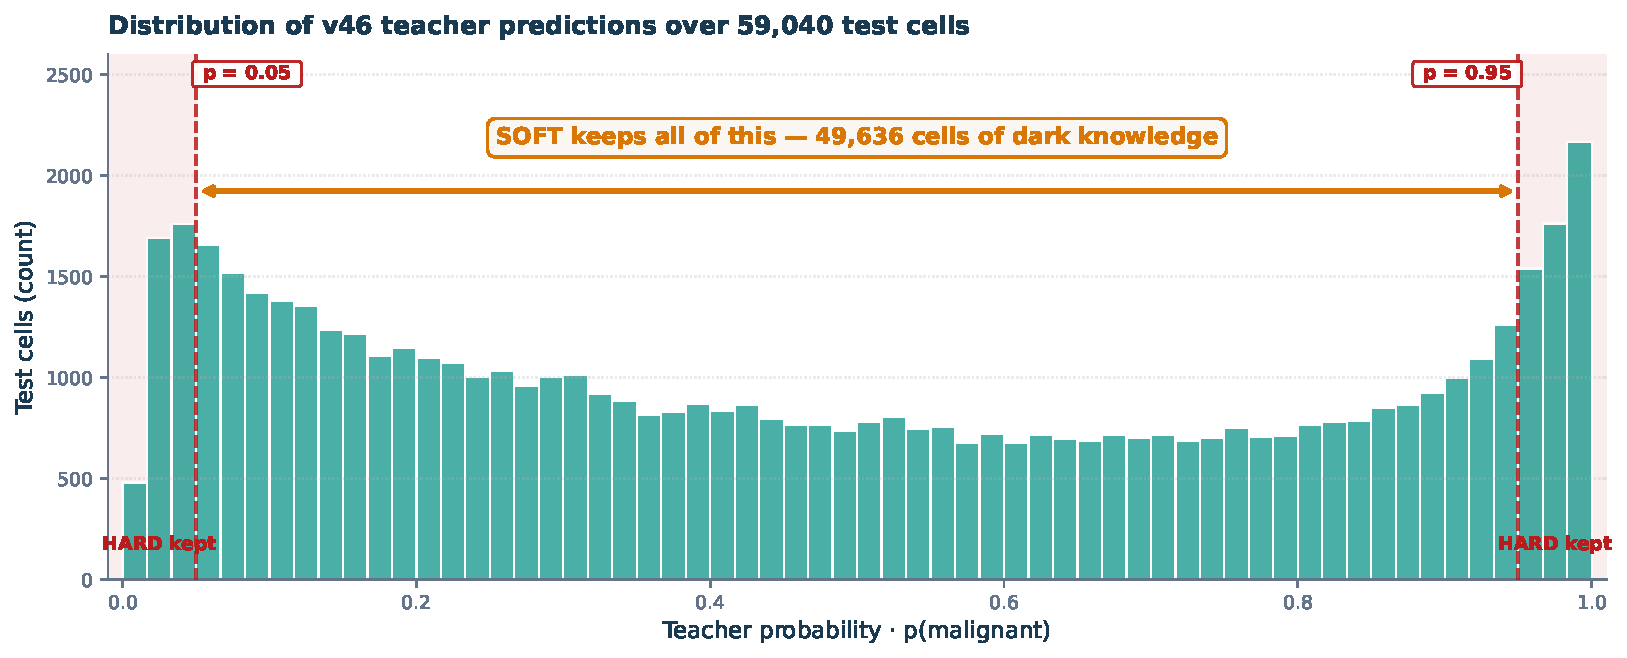
\includegraphics[width=0.95\textwidth]{teacher_prob_histogram.pdf}
  \caption{Teacher-probability histogram over all 59{,}040 test cells (v46 teacher). Crimson tails ($p < 0.05$ and $p > 0.95$) are the only cells that the Lee-2013 hard-pseudo recipe of v44 retains; v46 keeps all of the amber-band cells in between, weighting each by the teacher's raw probability.}
  \label{fig:hist}
\end{figure*}

\subsection{Iterative noisy student: mean lift compresses, dispersion expands}

v47 differs from v46 by exactly one variable: the pseudo-label CSV is v46's ensemble output (LB $0.8236$) instead of v44\_seed1's (LB $0.7844$). On the ensemble, round 2 lifts LB by $+0.003$ --- below the empirical seed noise floor ($\mathrm{SE}_\Delta = 0.0103$, see Table~\ref{tab:noisefloor}). The per-seed picture is more interesting and is summarized in Table~\ref{tab:seedspread}: the spread between best and worst seed widens from v46's $0.0072$ to v47's $0.0229$ ($3.2\times$ wider), the per-seed standard error widens from v46's $\mathrm{SE} = 0.0021$ to v47's $0.0073$ ($3.5\times$ larger), and the v47 ensemble underperforms its best single seed by $-0.0091$. We return to the within-recipe ensemble failure in \S\ref{sec:negative}-G.

\begin{table}[!t]
  \centering
  \caption{Per-seed and ensemble LB for the soft-pseudo (v46) and round-2 noisy-student (v47) families. The within-recipe ensemble is net-positive for v46 and net-negative for v47.}
  \label{tab:seedspread}
  \footnotesize
  \begin{tabular}{@{}lrrr@{}}
    \toprule
    Family & Worst seed & Best seed & Ensemble \\
    \midrule
    v46 & 0.8157 & 0.8229 & \textbf{0.8236} ($+0.0007$) \\
    v47 & 0.8126 & 0.8355 & 0.8264 ($-0.0091$) \\
    \midrule
    Seed range & --- & --- & --- \\
    v46 & \multicolumn{3}{r}{$0.0072$ \quad (3 seeds: $0.8157 / 0.8187 / 0.8229$)} \\
    v47 & \multicolumn{3}{r}{$0.0229$ \quad ($\sim$3$\times$ wider; per-seed SE $3.5\times$ larger)} \\
    \bottomrule
  \end{tabular}
\end{table}

\subsection{Other ablations}

\textbf{Backbone capacity at 128 native (v34 vs.\ v19).} ResNet-50 with the same recipe as v19 (no upscale, no discriminative LR) landed at $0.7155$, comparable to v23 (v19 with a different seed at $0.7154$). At $128$-pixel native input EfficientNet-B0 is not capacity-limited.

\textbf{Discriminative LR (v30).} The L4-textbook 1/10 backbone LR regressed by $\sim$$0.10$ LB. ImageNet-pretrained texture features need more LR to adapt to grayscale microscopy, not less; we kept a single global LR for the rest of the project.

\textbf{Within-recipe ensembling.} v44 ($0.7812$) was below its lucky single seed v44\_seed1 ($0.7844$); v46 ($0.8236$) beat all observed seeds; v47 ($0.8264$) underperformed its best seed by $0.0091$. The ensemble benefit is a function of seed-spread and outlier presence (\S\ref{sec:negative}-G).

\section{Negative Results and Failure-Mode Analysis}
\label{sec:negative}

We argue that the failure-mode diagnoses below are the most methodologically informative output of this project. Each subsection presents the experimental setup, the empirical result, the mechanism diagnosis, and the rule we adopted in response.

\subsection{v22 --- Cross-recipe sigmoid-averaging at a 0.05 LB gap}

\textbf{Setup.} Sigmoid-average of v19 ($0.7455$) and v21 ($0.7018$), under three weighting / averaging schemes: equal-weighted probability average, equal-weighted rank average, and LB-weighted probability average (member weights $\propto$ public LB).

\textbf{Result.} All three schemes underperformed v19 alone: $0.7422$ (equal-prob) / $0.7436$ (equal-rank) / $0.7328$ (LB-weighted) respectively.

\textbf{Diagnosis.} Sigmoid-averaging treats both members symmetrically. When members differ by more than the noise floor, the weaker model drags the ensemble below the stronger member on cells where they disagree. A non-uniform weighting (e.g., reciprocal-error) could in principle rescue this, but introduces a parameter that requires a non-trivial development set to fit.

\textbf{Rule.} Cross-recipe averaging is net-negative when members differ by more than $\sim$$0.02$ LB. We re-confirmed this on a tighter gap in v45\_probe (\S\ref{sec:negative}-F).

\subsection{v27 --- Single 2-patient held-out validation collapsed}

\textbf{Setup.} A 2-patient validation holdout (pat\_5 and pat\_14) with best-epoch selection on validation AUC.

\textbf{Result.} Best epoch selected was epoch 0 (random-init checkpoint). Public LB was correspondingly poor and the recipe was abandoned before further submissions.

\textbf{Diagnosis.} pat\_5 has saturated FL exposure and pat\_14 has unusually dim FL. With $N=12$ patients, removing two reduces the training-positive class to $\sim$10 patients of signal, and the held-out pair's adversarial brightness statistics drive validation AUC near random at every epoch. Best-epoch selection then locks onto the random-init checkpoint.

\textbf{Rule.} Conventional cross-validation does not work on $N=12$ patients with high per-patient distribution variance. We switched to using the public LB as the de-facto validation signal and accepted the 4-daily-submission quota as the rate-limiting cost.

\subsection{v37 / v38 --- Lian-paper transfer attempts}

\textbf{Setup.} v37: Lian \S5.2's modality-specific FL ColorJitter (brightness $0.8$, contrast $0.8$). v38: Lian Table 3's early fusion (concatenate BF and FL into a single 2-channel tensor fed to one backbone).

\textbf{Result.} v37 LB $0.7092$ ($-0.036$ from v19). v38 LB $0.7147$ ($-0.031$).

\textbf{Diagnosis.} Lian's FL is a 4-channel emission stack at higher resolution; ours is a 1-channel grayscale crop at $128 \times 128$. ColorJitter at brightness $0.8$ on an already-low-intensity grayscale signal removes most of the discriminative signal. Early fusion's benefit depends on per-pixel BF/FL alignment being tight enough to learn joint pixel-level features; on $128 \times 128$ paired crops the alignment is loose, so feature-level late fusion preserves more signal.

\textbf{Rule.} Re-validate borrowed ablations on the actual data modality and resolution before adopting them.

\subsection{v42 --- CoMIR-style SSL learned the patient shortcut}

\textbf{Setup.} CoMIR-style~\cite{pielawski2020comir} cross-modal InfoNCE pretrain: two encoders (BF and FL), shared projection head, positive pairs are paired (BF, FL) crops of the same cell. 10 epochs pretrain followed by 8 epochs of supervised finetune.

\textbf{Result.} InfoNCE loss converged to $0.02$ in epoch 1 (random baseline for 128-way contrastive is $\log 128 \approx 4.85$), then plateaued. Supervised finetune reached training-AUC $= 0.96$. Public LB: $0.5908$, near random.

\textbf{Diagnosis.} Each cell has exactly one source patient, so paired (BF, FL) of the same cell $i$ always share a patient. Unpaired (BF, FL) of cells $i, j$ with $i \ne j$ usually have different patients. The contrastive task is therefore solvable at $\ge 95\%$ accuracy by encoding the patient identity rather than the cell content; the pretrain backbone concentrates on the patient signature. The 0.4 gap between training AUC ($0.96$) and public LB ($0.59$) is the signature of the patient shortcut.

\textbf{Rule.} Cross-modal SSL on a strongly patient-grouped dataset can amplify the patient shortcut. To use it productively we would need positive pairs that span patient boundaries (e.g., two cells from different patients that share an annotated phenotype), which our annotations do not support.

\subsection{v43 --- four-component stack regressed $-0.012$}

\textbf{Setup.} v41 plus four simultaneous changes: (a) FL-tuned ColorJitter (brightness $0.5$, contrast $0.3$) $+$ RandomGamma $0.85$--$1.15$ on the FL branch only, (b) weight decay $10^{-4} \rightarrow 3\times 10^{-4}$, (c) 3-seed $\times$ SWA ensembling, (d) 40-way TTA replacing 24-way.

\textbf{Result.} LB $0.7444$, a $-0.012$ regression from v41.

\textbf{Submission-time diagnosis.} Unknown --- four changes were confounded.

\textbf{Retroactive diagnosis from v46.} v46 reverted (a) and (b) and added soft pseudo; the net gain over v43 was $+0.079$. Allowing soft pseudo to contribute the $+0.039$ we measured against v44\_seed1, the reverted components account for roughly $+0.04$ in net positive direction. The 3-seed $\times$ SWA ensemble and the extended TTA were kept across v44, v46, and v47 and are presumed beneficial in isolation.

\textbf{Rule.} Limit each submitted version to one or two related changes from the previous baseline. Stacking is methodologically expensive because it makes the component-isolation cost prohibitive on a 4-submission/day quota.

\subsection{v45\_probe --- cross-recipe ensemble at the tighter $0.025$ LB gap}

\textbf{Setup.} Local sigmoid-average of v41 ($0.7563$) and v44 ($0.7812$).

\textbf{Result.} LB $0.7729$. Below v44 alone by $0.0083$, but \emph{above} the naive linear LB-average ($0.76875$) by $0.0042$.

\textbf{Diagnosis.} The Pearson correlation between v41 and v44 predictions is $0.936$ --- the two prediction sets are correlated but not redundant; the ensemble adds small per-cell signal manifesting as a $+0.004$ lift above naive linear-LB-averaging. But the $0.025$-LB member gap is still wide enough that the weaker member's pull dominates the ensemble lift.

\textbf{Rule (refined).} Cross-recipe sigmoid-averaging at this dataset's scale is favorable only when member LB-gap is $\le 0.015$. Within-recipe ensembling (v44 / v46 / v47) remains the safe pattern in principle, though see the next subsection for an exception.

\subsection{v47 --- within-recipe ensemble net-negative under an outlier seed}

\textbf{Setup.} v47 trains 3 independent seeds of the iterative-noisy-student recipe and sigmoid-averages their TTA predictions. Each seed sees the same teacher (v46 ensemble) but with independent data shuffling, SWA epoch averaging, and random augmentation streams.

\textbf{Result.} Per-seed public LB: seed 1 $0.8150$, seed 2 $\mathbf{0.8355}$, seed 3 $0.8126$ (range $0.0229$). The 3-seed ensemble landed at $0.8264$, \emph{below} the best single seed by $0.0091$. By contrast, v46's per-seed range was $0.0072$ across 3 seeds ($0.8157 / 0.8187 / 0.8229$) and the v46 ensemble at $0.8236$ beat each individual seed. The ensemble shortfall is also observable on the public leaderboard: the v47\_s2 score holds $3$\textsuperscript{rd}, while the v47 ensemble would place $4$\textsuperscript{th}.

\textbf{Diagnosis.} The dynamic is identical to the cross-recipe collapse of \S\ref{sec:negative}-A and \S\ref{sec:negative}-F, but operating \emph{within} a single recipe at the seed level. Seed 2 is sufficiently strong on the public LB that averaging it with the two weaker seeds pulls the ensemble closer to their mean. There are two non-mutually-exclusive explanations: (i) seed 2 is a genuine outlier on the recipe's seed distribution and the ensemble is correctly hedging against its private-LB risk; (ii) seed 2 happened to land on a favorable public-LB sample and the ensemble's pull-toward-the-mean will be net-positive on the held-out private split.

\textbf{Implication for final-pick selection.} The two Kaggle private-LB submission slots admit three plausible strategies:
\begin{itemize}
  \item \emph{Aggressive:} v47 seed 2 ($0.8355$) $+$ v41 ($0.7563$ as a different-mechanism safety net).
  \item \emph{Robust:} v47 ensemble ($0.8264$) $+$ v41 ($0.7563$ as a different-mechanism safety net).
  \item \emph{Diversified within-pseudo:} v47 seed 2 $+$ v47 ensemble. No supervised-only safety net.
\end{itemize}
The robust strategy preserves the within-recipe averaging discipline of v46 but gives up $0.009$ public LB. The aggressive strategy bets that seed 2's training dynamics generalize; given v46's clean within-recipe averaging behavior at a tighter seed range, the seed-2 outlier may be public-LB-specific.

\textbf{Rule.} Within-recipe ensembling is not unconditionally net-positive. It is favorable when seed dispersion is tight relative to the underlying generalization gap. When one seed is a clear outlier, the ensemble can hedge against it correctly (private-LB-positive) or incorrectly (private-LB-negative); without a held-out signal it is not possible to decide between these in advance.

\subsection{Summary table}

Table~\ref{tab:failures} consolidates the seven diagnosed failures, their mechanisms, and whether the lesson was actioned in a subsequent version.

\begin{table}[!t]
  \centering
  \caption{Diagnosed failure modes and forward propagation of the lesson into subsequent versions.}
  \label{tab:failures}
  \footnotesize
  \begin{tabular}{@{}lp{4.5cm}c@{}}
    \toprule
    Failure & Mechanism diagnosed & Actioned? \\
    \midrule
    v22 & Cross-recipe ensemble at $0.05$ LB gap & yes \\
    v27 & 2-patient holdout too noisy on $N=12$ & yes \\
    v37 & FL ColorJitter strength too high for 1-channel grayscale & yes \\
    v38 & Early fusion needs tighter pixel alignment & yes \\
    v42 & Contrastive SSL learned patient identity, not cell content & yes \\
    v43 & Four-change stack confounded; $\ge 1$ component net-negative & yes \\
    v45\_probe & Cross-recipe ensemble fails at $0.025$ gap & yes \\
    v47 & Within-recipe ensemble net-negative under outlier seed & open \\
    \bottomrule
  \end{tabular}
\end{table}

\section{Discussion}
\label{sec:discussion}

\subsection{The dataset-size lever dominates architecture and regularization}

The v19$\rightarrow$v41 stack of four textbook regularizers (label smoothing, dropout, paired RandomResizedCrop, multiscale TTA) returned $+0.011$ LB. The single change ``add $\sim$9{,}400 confident test cells with hard labels'' returned $+0.025$ LB. The single change ``use all 59{,}040 test cells with raw probability targets'' returned $+0.039$ LB. With 12 patients and 114k labeled cells the model is data-bound, not capacity-bound; methods that effectively grow the labeled set dominate methods that polish the supervised loss surface, by an order of magnitude in this regime.

\subsection{Why soft pseudo beat hard pseudo so dramatically}

Hard pseudo at threshold $0.05/0.95$ discards 84\% of test cells (49{,}640 of 59{,}040; see Fig.~\ref{fig:hist}). Soft pseudo keeps all 59{,}040, weighting each cell's contribution by the teacher's confidence. Hinton's ``dark knowledge'' argument~\cite{hinton2015distilling} applies cleanly: a cell labeled $p_t = 0.78$ by the teacher carries both directional and magnitude information that hard binarization throws away. On this benchmark the per-cell expected information appears to be larger than the noise from incorrect teacher predictions in the intermediate-confidence band, even though many of those soft labels are individually wrong.

\subsection{Iterative noisy student: where does the round-2 lift actually go?}

Round 1 (v44 hard $\rightarrow$ v46 soft) returned $+0.039$ LB. Round 2 (v46 soft $\rightarrow$ v47 soft with v46 ensemble as teacher) returned $+0.003$ LB on the ensemble. The mean lift compressed $\sim$14$\times$. Two observations:

\emph{The mean compresses, the per-seed dispersion expands.} The v47 per-seed LB range ($0.8126$--$0.8355$, span $0.0229$) is $3.2\times$ wider than v46's ($0.8157$--$0.8229$, span $0.0072$, both at $n=3$). Equivalently, v47's per-seed public-LB standard error ($\mathrm{SE} = 0.0073$) is $3.5\times$ larger than v46's ($\mathrm{SE} = 0.0021$). This is the inverse of what an earlier draft of this paper hypothesized (``round 2 acts as a variance reducer''); the training-AUC tightened but the generalization spread widened. The empirically correct framing is that round 2 with a much-stronger teacher creates a higher-variance student distribution, with seed-2 landing on a favorable mode of that distribution.

\emph{The diminishing-returns regime starts after one round.} Round 1 unlocks the calibration channel that hard pseudo discards; subsequent rounds re-iterate the same channel with a marginally better-calibrated teacher. To extract a further mean lift one would need to change the mechanism, not the iteration count --- for instance, softening the teacher distribution via Hinton's temperature parameter, introducing stronger student-side input/dropout noise, or (the direction our subsequent runs take) adding \emph{architectural} diversity so that a cross-architecture ensemble can exceed the best single recipe (\S\ref{sec:discussion}-D).

\subsection{When ensembling helps and when it does not}

Three regimes appeared in the data:
\begin{itemize}
  \item \emph{Within-recipe, tight seed dispersion} (v46): ensemble beats all observed seeds.
  \item \emph{Within-recipe, wide seed dispersion with one outlier} (v47): ensemble underperforms the outlier seed.
  \item \emph{Cross-recipe} (v22, v45\_probe): ensemble underperforms the stronger member whenever the LB gap exceeds $\sim$$0.015$--$0.02$.
\end{itemize}
The common mechanism is that sigmoid-averaging is symmetric; whenever one member is substantially stronger on the evaluation distribution than the others, symmetric averaging pulls the ensemble toward the weaker members. The cure --- non-uniform weights --- requires a development set that the patient-disjoint structure (\S\ref{sec:negative}-B) does not afford.

\textbf{Implication for future work: diversify the backbone, not the seed.} Every strong model in this study shares the EfficientNet-B0 dual-branch backbone, so their predictions are highly correlated (rank-correlation $>0.94$ among v44/v46/v47) --- which is precisely why symmetric averaging never beats the best single seed here. The route to a net-positive ensemble is therefore \emph{architectural} diversity: members that are individually strong but decorrelated. A rank-correlation analysis over our archived submissions identifies the most promising decorrelated bases --- an \emph{early-fusion} single backbone on the stacked 2-channel input (rank-corr $0.72$ with our best model) and a \emph{ResNet-50} backbone (rank-corr $0.80$) --- both currently weak only because they were trained supervised-only. Re-training these (and a ConvNeXt variant) under the soft-pseudo recipe and blending across backbone families is the natural next step, and the one averaging regime the analysis above predicts can actually help.

\subsection{Limitations and threats to validity}

\textbf{Single public-LB number per submission.} Each LB delta in this paper is a single noisy estimate from one public-LB split. The three submitted v47 seeds give a direct empirical noise-floor measurement: $\mathrm{SE}_{v47} = 0.0073$ (mean $0.8210$, sample SD $0.0126$ across LBs $\{0.8126, 0.8150, 0.8355\}$). For comparison, v46's three seeds give $\mathrm{SE}_{v46} = 0.0021$ (SD $0.0036$ across $\{0.8157, 0.8187, 0.8229\}$): v47's seed noise is $3.5\times$ larger, evidence that round-2 noisy student widens rather than narrows the student distribution. Treating each version's LB as a single noisy observation with the (conservative) v47 SE, the SE of a paired delta is $\mathrm{SE}_\Delta = \sqrt{2} \cdot \mathrm{SE}_{v47} = 0.0103$. Table~\ref{tab:noisefloor} expresses each headline delta as a multiple of this $\mathrm{SE}_\Delta$, alongside two prediction-level stability statistics (Pearson $r$ between ensemble probability outputs, and the per-cell sigmoid-sign-flip rate). The v44$\rightarrow$v46 soft-pseudo gain at $4.13\sigma$ is the only \emph{robust} delta; the v41$\rightarrow$v44 hard-pseudo gain at $2.42\sigma$ is supported; the v19$\rightarrow$v41 regularizer-stack gain at $1.05\sigma$ is marginal; the v46$\rightarrow$v47 round-2 ensemble gain at $0.27\sigma$ is \emph{indistinguishable from zero} at this noise floor. We note further that the within-v47 cross-seed sigmoid-sign-flip rate ($12.6\%$ averaged across the three seed pairs) is \emph{larger} than the v46$\rightarrow$v47 ensemble cross-version flip rate ($4.0\%$); seed-level variation dominates round-2 signal.

\textbf{Where does v47\_s2's lift over the ensemble actually come from?} A per-cell analysis of v47\_s2 versus the v47 ensemble (both trained against the same v46 ensemble teacher) shows that $97\%$ of total $|p_{s2} - p_{ens}|$ is concentrated in the $84\%$ of test cells where the v46 teacher predicted $p \in [0.05, 0.95]$ --- the ``dark knowledge'' middle band of teacher uncertainty. The remaining $16\%$ of cells (the confident-teacher tails) contribute only $3\%$ of total disagreement. Stratified by v47 ensemble confidence decile, the sign-flip rate is $0$--$1\%$ in deciles D1--D5 and D8--D10 (cells the ensemble was confident about) and $33$--$58\%$ in D6--D7 (cells with ensemble probability between $0.46$ and $0.72$). The two predictors agree on every confident class call and diverge sharply on exactly the cells where there is genuine ambiguity. This is consistent with seed-2's lift being signal rather than public-split luck: s2 found a more decisive boundary in the teacher's uncertain region, rather than overriding confident predictions. Whether this signal generalizes to the private LB split remains the central open question for the final-pick decision (\S\ref{sec:negative}-G).

% Auto-generated by overleaf-report/figure-sources/build_noise_floor_analysis.py
% Headline-delta significance test against the v47 per-seed noise floor.
\begin{table}[!t]
  \centering
  \caption{Headline LB deltas with prediction-level stability statistics. $\mathrm{SE}_\Delta = \sqrt{2} \cdot \mathrm{SE}_{v47}$ $= 0.0103$, using the v47 per-seed SE (0.0073) as a conservative single-seed noise estimate. Pearson $r$ is between ensemble probability outputs over the 59{,}040 test cells; flip\% is the fraction of cells where the sigmoid sign disagrees between the two versions.}
  \label{tab:noisefloor}
  \footnotesize
  \begin{tabular}{@{}lrrrrl@{}}
    \toprule
    Pair & $\Delta$LB & Pearson $r$ & Flip\% & $|\Delta|/\mathrm{SE}_\Delta$ & Verdict \\
    \midrule
    v19 $\to$ v41 & $+0.0108$ & $0.854$ & $14.43\%$ & $+1.05$ & marginal ($\ge 1\sigma$) \\
    v41 $\to$ v44 & $+0.0249$ & $0.936$ & $9.53\%$ & $+2.42$ & supported ($\ge 2\sigma$) \\
    v44 $\to$ v46 & $+0.0424$ & $0.963$ & $9.22\%$ & $+4.13$ & \textbf{robust} ($\ge 4\sigma$) \\
    v44\_seed1 $\to$ v46 & $+0.0392$ & $0.957$ & $9.22\%$ & $+3.81$ & supported ($\ge 2\sigma$) \\
    v46 $\to$ v47 & $+0.0028$ & $0.990$ & $3.99\%$ & $+0.27$ & indistinguishable ($<1\sigma$) \\
    v46 $\to$ v47\_seed2 & $+0.0119$ & $0.967$ & $9.00\%$ & $+1.16$ & marginal ($\ge 1\sigma$) \\
    \bottomrule
  \end{tabular}
\end{table}


\textbf{Possible overfitting to public LB.} Aggressive iteration on a single LB signal risks tailoring to the public split. v41 (the strongest non-pseudo baseline) is kept as the safety pick precisely because it shares no pseudo-label lineage with the v44/v46/v47 chain.

\textbf{Generalization beyond this dataset.} The dataset-size dominance argument depends on the small-$N$ patient-grouped structure. We expect the relative ordering ``soft pseudo $>$ hard pseudo $>$ supervised regularization'' to be specific to similar regimes (few patients, many cells per patient, patient-disjoint test set); on natural-image benchmarks with many independent training subjects the ordering may invert.

\subsection{What did \emph{not} work and why}

The seven negative results in \S\ref{sec:negative} fall into three families. Cross-recipe and outlier-within-recipe averaging fail when member quality is asymmetric (\S\ref{sec:negative}-A, F, G). Standard model-selection machinery (single held-out fold, discriminative LR, modality-specific augmentation strengths borrowed from related work) fails because it does not transfer cleanly to the small-$N$ / 1-channel-grayscale / $128 \times 128$ regime (\S\ref{sec:negative}-B, C, E). Cross-modal SSL fails because the contrastive task admits a trivial patient-identity solution under the per-cell patient assignment (\S\ref{sec:negative}-D). None of these failures was predictable from the textbook --- each required running the experiment to surface.

\section{Conclusion}
\label{sec:conclusion}

Across 30 logged iterations on a small-sample patient-grouped multimodal-microscopy benchmark, we layered EfficientNet-B0 dual-branch architecture, MIL auxiliary loss, batch-normalization adaptation, multiscale TTA, label-smoothing and dropout regularization, hard pseudo-labels, soft-target distillation, and iterative noisy student training. The public-LB lift over a strong supervised baseline (v19 $0.7455$ $\rightarrow$ v47 ensemble $0.8264$ / best seed $0.8355$) is $+0.081$--$+0.090$. The single largest gain ($+0.042$ LB, $4.13\sigma$ relative to the seed noise floor) is from soft pseudo-labels replacing hard, and is one order of magnitude larger than the cumulative regularizer-stack gain. The round-2 noisy-student gain ($+0.003$ ensemble, $0.27\sigma$) is below the noise floor and is treated as a saturation rather than a continued improvement. At submission time the best-seed score holds $3$\textsuperscript{rd} on the public leaderboard, $\sim$$0.009$ behind the first two teams. Seven failure modes are diagnosed, including a within-recipe ensemble net-negative under an outlier seed that informs the final-pick decision.

Three take-aways:
\begin{enumerate}
  \item On small-$N$ patient-grouped microscopy, growing the \emph{effective} labeled set via test-set pseudo-labels and distillation outperforms architectural and regularization gains by an order of magnitude.
  \item Sigmoid-averaging is symmetric: whether cross-recipe or within-recipe-with-outlier, the ensemble underperforms the strong member when member quality is asymmetric. The cure (non-uniform weights) requires a held-out signal that the patient-disjoint structure does not afford.
  \item Negative results carry more methodological signal than the wins on a benchmark this small. The seven diagnoses in \S\ref{sec:negative} are what shaped the recipe; the LB number is a consequence.
\end{enumerate}

\section*{Acknowledgments}

Conducted as Assignment~3 of the Uppsala University course \emph{1MD042 Advanced Deep Learning for Image Processing} (Spring 2026). The author thanks the course instructor for the open-tooling policy that made the pseudo-label and distillation experiments possible within the course timeline.

\bibliographystyle{IEEEtran}
\bibliography{refs}

\end{document}
